%% abtex2-modelo-trabalho-academico.tex, v-1.9.7 laurocesar
%% Copyright 2012-2018 by abnTeX2 group at http://www.abntex.net.br/ 
%%
%% This work may be distributed and/or modified under the
%% conditions of the LaTeX Project Public License, either version 1.3
%% of this license or (at your option) any later version.
%% The latest version of this license is in
%%   http://www.latex-project.org/lppl.txt
%% and version 1.3 or later is part of all distributions of LaTeX
%% version 2005/12/01 or later.
%%
%% This work has the LPPL maintenance status `maintained'.
%% 
%% The Current Maintainer of this work is the abnTeX2 team, led
%% by Lauro César Araujo. Further information are available on 
%% http://www.abntex.net.br/
%%
%% This work consists of the files abntex2-modelo-trabalho-academico.tex,
%% abntex2-modelo-include-comandos and abntex2-modelo-references.bib
%%

% ------------------------------------------------------------------------
% ------------------------------------------------------------------------
% abnTeX2: Modelo de Trabalho Academico (tese de doutorado, dissertacao de
% mestrado e trabalhos monograficos em geral) em conformidade com 
% ABNT NBR 14724:2011: Informacao e documentacao - Trabalhos academicos -
% Apresentacao
% ------------------------------------------------------------------------
% ------------------------------------------------------------------------

\documentclass[
	% -- opções da classe memoir --
	12pt,				% tamanho da fonte
	openright,			% capítulos começam em pág ímpar (insere página vazia caso preciso)
	twoside,			% para impressão em recto e verso. Oposto a oneside
	a4paper,			% tamanho do papel. 
	% -- opções da classe abntex2 --
	%chapter=TITLE,		% títulos de capítulos convertidos em letras maiúsculas
	%section=TITLE,		% títulos de seções convertidos em letras maiúsculas
	%subsection=TITLE,	% títulos de subseções convertidos em letras maiúsculas
	%subsubsection=TITLE,% títulos de subsubseções convertidos em letras maiúsculas
	% -- opções do pacote babel --
	english,			% idioma adicional para hifenização
	brazil				% o último idioma é o principal do documento
	]{abntex2}

% ---
% Pacotes básicos 
% ---
\usepackage{lmodern}			% Usa a fonte Latin Modern			
\usepackage[T1]{fontenc}		% Selecao de codigos de fonte.
\usepackage[utf8]{inputenc}		% Codificacao do documento (conversão automática dos acentos)
\usepackage{indentfirst}		% Indenta o primeiro parágrafo de cada seção.
\usepackage{color}				% Controle das cores
\usepackage{graphicx}			% Inclusão de gráficos
\usepackage{microtype} 			% para melhorias de justificação
% ---
		
% ---
% Pacotes adicionais, usados apenas no âmbito do Modelo Canônico do abnteX2
% ---
\usepackage{lipsum}				% para geração de dummy text
% ---

% ---
% Pacotes de citações
% ---
\usepackage[brazilian,hyperpageref]{backref}	 % Paginas com as citações na bibl
\usepackage[alf]{abntex2cite}	% Citações padrão ABNT
\citebrackets()

% --- 
% CONFIGURAÇÕES DE PACOTES
% --- 

% ---
% Configurações do pacote backref
% Usado sem a opção hyperpageref de backref
\renewcommand{\backrefpagesname}{Citado na(s) página(s):~}
% Texto padrão antes do número das páginas
\renewcommand{\backref}{}
% Define os textos da citação
\renewcommand*{\backrefalt}[4]{
	\ifcase #1 %
		Nenhuma citação no texto.%
	\or
		Citado na página #2.%
	\else
		Citado #1 vezes nas páginas #2.%
	\fi}%
% ---

% ---
% Informações de dados para CAPA e FOLHA DE ROSTO
% ---
\titulo{Modelo de Trabalho de Trabalho Acadêmico da Faculdade de Computação e Programa de Pós-Graduação em Ciência da Computação.}
\autor{Jairo Nascimento de Sousa Filho}
\local{Belém}
\data{2019}
\orientador{Prof. Dr. Carlos Gustavo Resque dos Santos}
\coorientador{}
\instituicao{Universidade Federal do Pará}
\instituicaounidade{Instituto de Ciências Exatas e Naturais}
\instituicaosubunidade{Faculdade de Computação}


\tipotrabalho{Monografia (Graduação)}
% O preambulo deve conter o tipo do trabalho, o objetivo, 
% o nome da instituição e a área de concentração 
\preambulo{Monografia apresentada na Faculdade de Computação do Instituto de Ciências Exatas e Naturais como requisito parcial para obtenção do grau de Bacharel.}
% ---


% ---
% Configurações de aparência do PDF final

% alterando o aspecto da cor azul
\definecolor{blue}{RGB}{41,5,195}

% informações do PDF
\makeatletter
\hypersetup{
     	%pagebackref=true,
		pdftitle={\@title}, 
		pdfauthor={\@author},
    	pdfsubject={\imprimirpreambulo},
	    pdfcreator={LaTeX with abnTeX2},
		pdfkeywords={abnt}{latex}{abntex}{abntex2}{trabalho acadêmico}, 
		colorlinks=true,       		% false: boxed links; true: colored links
    	linkcolor=black,          	% color of internal links
    	citecolor=black,        		% color of links to bibliography
    	filecolor=black,      		% color of file links
		urlcolor=black,
		bookmarksdepth=4
}
\makeatother
% --- 

% ---
% Posiciona figuras e tabelas no topo da página quando adicionadas sozinhas
% em um página em branco. Ver https://github.com/abntex/abntex2/issues/170
\makeatletter
\setlength{\@fptop}{5pt} % Set distance from top of page to first float
\makeatother
% ---

% ---
% Possibilita criação de Quadros e Lista de quadros.
% Ver https://github.com/abntex/abntex2/issues/176
%
\newcommand{\quadroname}{Quadro}
\newcommand{\listofquadrosname}{Lista de quadros}

\newfloat[chapter]{quadro}{loq}{\quadroname}
\newlistof{listofquadros}{loq}{\listofquadrosname}
\newlistentry{quadro}{loq}{0}

% configurações para atender às regras da ABNT
\setfloatadjustment{quadro}{\centering}
\counterwithout{quadro}{chapter}
\renewcommand{\cftquadroname}{\quadroname\space} 
\renewcommand*{\cftquadroaftersnum}{.\hfill}

\setfloatlocations{quadro}{hbtp} % Ver https://github.com/abntex/abntex2/issues/176
% ---

% --- 
% Espaçamentos entre linhas e parágrafos 
% --- 

% O tamanho do parágrafo é dado por:
\setlength{\parindent}{1.3cm}

% Controle do espaçamento entre um parágrafo e outro:
\setlength{\parskip}{0.2cm}  % tente também \onelineskip

% ---
% compila o indice
% ---
\makeindex
% ---

% ----
% Início do documento
% ----
\begin{document}

% Seleciona o idioma do documento (conforme pacotes do babel)
%\selectlanguage{english}
\selectlanguage{brazil}

% Retira espaço extra obsoleto entre as frases.
\frenchspacing 

% ----------------------------------------------------------
% ELEMENTOS PRÉ-TEXTUAIS
% ----------------------------------------------------------
% \pretextual

% ---
% Capa
% ---
\imprimircapa
% ---

% ---
% Folha de rosto
% (o * indica que haverá a ficha bibliográfica)
% ---
\imprimirfolhaderosto*
% ---

% ---
% Inserir a ficha bibliografica
% ---

% Isto é um exemplo de Ficha Catalográfica, ou ``Dados internacionais de
% catalogação-na-publicação''. Você pode utilizar este modelo como referência. 
% Porém, provavelmente a biblioteca da sua universidade lhe fornecerá um PDF
% com a ficha catalográfica definitiva após a defesa do trabalho. Quando estiver
% com o documento, salve-o como PDF no diretório do seu projeto e substitua todo
% o conteúdo de implementação deste arquivo pelo comando abaixo:
%
% \begin{fichacatalografica}
%     \includepdf{fig_ficha_catalografica.pdf}
% \end{fichacatalografica}

\begin{fichacatalografica}
	\sffamily
	\vspace*{\fill}					% Posição vertical
	\begin{center}					% Minipage Centralizado
	\fbox{\begin{minipage}[c][8cm]{13.5cm}		% Largura
	\small
	Solicite sua ficha catalográfica em: \url{http://bcficat.ufpa.br/}
	\end{minipage}}
	\end{center}
\end{fichacatalografica}
% ---

% ---
% Inserir errata
% ---
%\begin{errata}
%Elemento opcional da %\cite{NBR14724:2011}. Exemplo:

%\vspace{\onelineskip}

%FERRIGNO, C. R. A. \textbf{Tratamento de neoplasias ósseas apendiculares com
%reimplantação de enxerto ósseo autólogo autoclavado associado ao plasma
%rico em plaquetas}: estudo crítico na cirurgia de preservação de membro em
%cães. 2011. 128 f. Tese (Livre-Docência) - Faculdade de Medicina Veterinária e
%Zootecnia, Universidade de São Paulo, São Paulo, 2011.

%\begin{table}[htb]
%\center
%\footnotesize
%\begin{tabular}{|p{1.4cm}|p{1cm}|p{3cm}|p{3cm}|}
%  \hline
%   \textbf{Folha} & \textbf{Linha}  & \textbf{Onde se lê}  & \textbf{Leia-se}  \\
%    \hline
%    1 & 10 & auto-conclavo & autoconclavo\\
%   \hline
%\end{tabular}
%\end{table}

%\end{errata}
% ---

% ---
% Inserir folha de aprovação
% ---

% Isto é um exemplo de Folha de aprovação, elemento obrigatório da NBR
% 14724/2011 (seção 4.2.1.3). Você pode utilizar este modelo até a aprovação
% do trabalho. Após isso, substitua todo o conteúdo deste arquivo por uma
% imagem da página assinada pela banca com o comando abaixo:
%
% \begin{folhadeaprovacao}
% \includepdf{folhadeaprovacao_final.pdf}
% \end{folhadeaprovacao}
%
\begin{folhadeaprovacao}

  \begin{center}
    {\ABNTEXchapterfont\large\imprimirautor}

    \vspace*{\fill}\vspace*{\fill}
    \begin{center}
      \ABNTEXchapterfont\bfseries\Large\imprimirtitulo
    \end{center}
    \vspace*{\fill}
    
    \hspace{.45\textwidth}
    \begin{minipage}{.5\textwidth}
        \imprimirpreambulo
    \end{minipage}%
    \vspace*{\fill}
   \end{center}
        
   Conceito: Excelente!\rule{3cm}{.1pt}
   
   \imprimirlocal, 1 de janeiro de 2019.
   
   \vspace{1cm}
   \begin{center}
   BANCA EXAMINADORA
   \end{center}
    

   \assinatura{\textbf{\imprimirorientador} - Orientador \\ UFPA}
   %\assinatura{\textbf{\imprimircoorientador} - Coorientador \\ UFPA}
   \assinatura{\textbf{Nome Convidado 1} \\ SIGLA INSTITUIÇÃO}
   \assinatura{\textbf{Nome Convidado 2} \\ SIGLA INSTITUIÇÃO}
   %\assinatura{\textbf{Nome Convidado 3} \\ SIGLA INSTITUIÇÃO}
      

  
\end{folhadeaprovacao}
% ---

% ---
% Dedicatória
% ---
\begin{dedicatoria}
   \vspace*{\fill}
   \centering
   \noindent
   \textit{ Escreva sua dedicatória aqui.} \vspace*{\fill}
\end{dedicatoria}
% ---

% ---
% Agradecimentos
% ---
\begin{agradecimentos}
Os agradecimentos principais são direcionados à Gerald Weber, Miguel Frasson,
Leslie H. Watter, Bruno Parente Lima, Flávio de Vasconcellos Corrêa, Otavio Real
Salvador, Renato Machnievscz e todos aqueles que
contribuíram para que a produção de trabalhos acadêmicos conforme
as normas ABNT com \LaTeX\ fosse possível.

Agradecimentos especiais são direcionados ao Centro de Pesquisa em Arquitetura
da Informação da Universidade de
Brasília (CPAI), ao grupo de usuários
\emph{latex-br} e aos
novos voluntários do grupo
\emph{\abnTeX} e que contribuíram e que ainda
contribuirão para a evolução do \abnTeX.

\end{agradecimentos}
% ---

% ---
% Epígrafe
% ---
\begin{epigrafe}
    \vspace*{\fill}
	\begin{flushright}
		\textit{``Escreva sua epígrafe aqui''\\
		(Fulano de Tal, 19XX)}
	\end{flushright}
\end{epigrafe}
% ---

% ---
% RESUMOS
% ---

% resumo em português
\setlength{\absparsep}{18pt} % ajusta o espaçamento dos parágrafos do resumo
\begin{resumo}
 Segundo a \cite{NBR6028:2003}, o resumo deve ressaltar o
 objetivo, o método, os resultados e as conclusões do documento. A ordem e a extensão
 destes itens dependem do tipo de resumo (informativo ou indicativo) e do
 tratamento que cada item recebe no documento original. O resumo deve ser
 precedido da referência do documento, com exceção do resumo inserido no
 próprio documento. (\ldots) As palavras-chave devem figurar logo abaixo do
 resumo, antecedidas da expressão Palavras-chave:, separadas entre si por
 ponto e finalizadas também por ponto.

 \textbf{Palavras-chave}: latex. abntex. editoração de texto.
\end{resumo}

% resumo em inglês
\begin{resumo}[Abstract]
 \begin{otherlanguage*}{english}
   This is the english abstract.

   \vspace{\onelineskip}
 
   \noindent 
   \textbf{Keywords}: latex. abntex. text editoration.
 \end{otherlanguage*}
\end{resumo}

% ---

% ---
% inserir lista de ilustrações
% ---
\pdfbookmark[0]{\listfigurename}{lof}
\listoffigures*
\cleardoublepage
% ---

% ---
% inserir lista de quadros
% ---
\pdfbookmark[0]{\listofquadrosname}{loq}
\listofquadros*
\cleardoublepage
% ---

% ---
% inserir lista de tabelas
% ---
\pdfbookmark[0]{\listtablename}{lot}
\listoftables*
\cleardoublepage
% ---

% ---
% inserir lista de abreviaturas e siglas
% ---
\begin{siglas}
  \item[ABNT] Associação Brasileira de Normas Técnicas
  \item[abnTeX] ABsurdas Normas para TeX
\end{siglas}
% ---

% ---
% inserir lista de símbolos
% ---
\begin{simbolos}
  \item[$ \Gamma $] Letra grega Gama
  \item[$ \Lambda $] Lambda
  \item[$ \zeta $] Letra grega minúscula zeta
  \item[$ \in $] Pertence
\end{simbolos}
% ---

% ---
% inserir o sumario
% ---
\pdfbookmark[0]{\contentsname}{toc}
\tableofcontents*
\cleardoublepage
% ---



% ----------------------------------------------------------
% ELEMENTOS TEXTUAIS
% ----------------------------------------------------------
\textual

% ----------------------------------------------------------
% Introdução (exemplo de capítulo sem numeração, mas presente no Sumário)
% ----------------------------------------------------------
\chapter{Introdução}
% ----------------------------------------------------------
%Mostrar o que são dados sintéticos de forma geral.
%Mostrar o problema que é a utilização de dados reais.
%Mostrar o uso de dados sintéticos e principais locais de uso.
%Mostrar a necessidade de um gerador de dados sintéticos.
%Mostrar que já existem geradores de dados sintéticos.
%Mostrar o diferencial do protótipo que procuramos fazer.

Este documento e seu código-fonte são exemplos de referência de uso da classe
\textsf{abntex2} e do pacote \textsf{abntex2cite}. O documento 
exemplifica a elaboração de trabalho acadêmico (tese, dissertação e outros do
gênero) produzido conforme a ABNT NBR 14724:2011 \emph{Informação e documentação
- Trabalhos acadêmicos - Apresentação}.

A expressão ``Modelo Canônico'' é utilizada para indicar que \abnTeX\ não é
modelo específico de nenhuma universidade ou instituição, mas que implementa tão
somente os requisitos das normas da ABNT. Uma lista completa das normas
observadas pelo \abnTeX\ é apresentada em \cite{abntex2classe}.

Sinta-se convidado a participar do projeto \abnTeX! Acesse o site do projeto em
\url{http://www.abntex.net.br/}. Também fique livre para conhecer,
estudar, alterar e redistribuir o trabalho do \abnTeX, desde que os arquivos
modificados tenham seus nomes alterados e que os créditos sejam dados aos
autores originais, nos termos da ``The \LaTeX\ Project Public
License''\footnote{\url{http://www.latex-project.org/lppl.txt}}.

Encorajamos que sejam realizadas customizações específicas deste exemplo para
universidades e outras instituições --- como capas, folha de aprovação, etc.
Porém, recomendamos que ao invés de se alterar diretamente os arquivos do
\abnTeX, distribua-se arquivos com as respectivas customizações.
Isso permite que futuras versões do \abnTeX~não se tornem automaticamente
incompatíveis com as customizações promovidas. Consulte
\cite{abntex2-wiki-como-customizar} para mais informações.

Este documento deve ser utilizado como complemento dos manuais do \abnTeX\ 
\cite{abntex2classe,abntex2cite,abntex2cite-alf} e da classe \textsf{memoir}
\cite{memoir}. 

Esperamos, sinceramente, que o \abnTeX\ aprimore a qualidade do trabalho que
você produzirá, de modo que o principal esforço seja concentrado no principal:
na contribuição científica.

Equipe \abnTeX 

Lauro César Araujo

% ---
\chapter{Fundamentação Teórica}\label{cap_exemplos}
% ---

	% Por que estou fazendo isso?
	% Qual a necessidade de um gerador de dados sintéticos?
	% Já existem aplicações? Quais os seus prós e contras?
	% Onde são aplicados os dados sintéticos.
	% Qual o desempenho? Quais os resultados? Discussão.

	% Escrever um overview. Principais funcionalidades. Multiplataforma. Forma de pagamento.
	% Funcionalidades Detalhadas.
	% Se houver softwares relacionados, explicar um pouco mais sobre.
	% Mostrar a foto.

	\section{Dados Sintéticos}
	O conceito de geração de dados sintéticos vieram por volta de 1993, por Rubin. \cite{rubin1993statistical}
	Em suma, seu objetivo era tonar anônimo os domicílios que participaram do censo daquela época.
	A partir desse fato, confidencialidade dos dados se tornou muito necessário, o que ajudou na popularização dos dados sintéticos.
	Portanto, dados sintéticos foi definido como "qualquer dado produzido o qual possa ser aplicado a uma dada situação que não foi obtido por mensuração direta.". \cite{mcgraw-hilleducation2016}
	\par
	A necessidade de dados sintéticos podem ser de várias formas, 
	desde a escassez de dados reais ou indisponibilidade;
	 para teste de dados não usuais;
	 para evitar lidar com questões de privacidade dos dados;
	 teste de aplicação sem precisar modificar dados da aplicação de produção;
	 criar teste de estresse da aplicação com \emph{Big Data} antes de criar versão para produção;
	 bem como não precisar adicionar os dados de teste manualmente. \cite{top15DatagenTools2019}
	\par
	A aplicabilidade dos dados sintéticos é ilimitada, e é bastante explorada por setores cujos dados são sensíveis como a financeiro \cite{lopez2012money} e de saúde. \cite{bergeat2014french} 	
	Também são muito bem aplicáveis para exaustívos testes de segurança, os quais são necessários vários casos de teste, já que o pesquisador tem controle suficiente processamento (fórmulas matemáticas ou regras de geração) e saída do dado, como um sistema de detecção de fraudes. \cite{barse2003synthesizing}
	 
	\subsection{Trabalhos Relacionados}
	\begin{figure}
		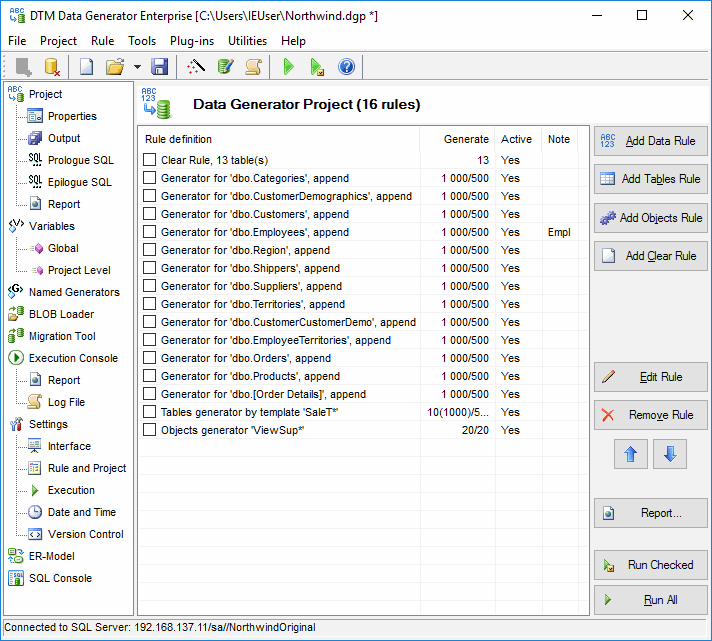
\includegraphics[width=\linewidth]{./figures/TrabalhosRelacionados/DTMDataGenerator.png}
		\caption{Usando o DTM Data Generator. Fonte: DTM Data Generator}
		\label{fig:DTMDG}
	\end{figure}
	\begin{figure}
		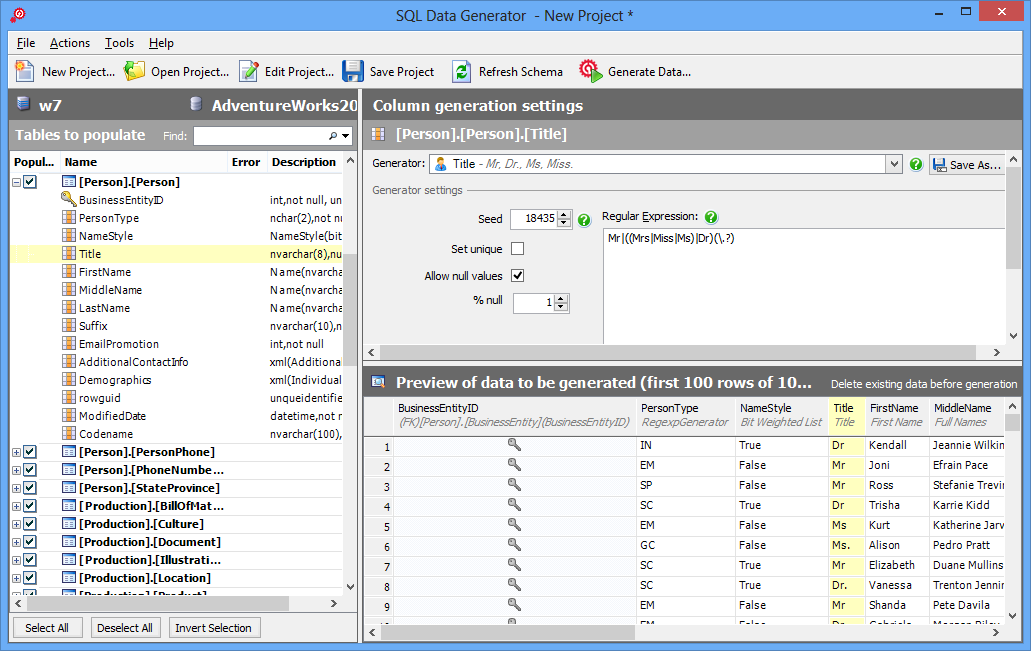
\includegraphics[width=\linewidth]{./figures/TrabalhosRelacionados/sql-data-generator.png}
		\caption{Usando o Redgate SQL Data Generator. Fonte: Red Gate SQL Data Generator}
		\label{fig:RedgateSQLDG}
	\end{figure}
	\subsubsection{DTM Data Generator}
	DTM Data Generator \cite{DTMDataGenerator} é uma plataforma de geração de dados sintéticos que existe de 1998.
	Esta possui suporte para geração de dados em arquivos, em banco de dados, também para \emph{Big Data}.
	Possui suporte multiplataforma, através do modo \emph{multiplatform runtime}, contudo é limitado quando comparado à versão Windows, o qual suporta a versão para servidor também.
	É válido destacar que é um software essencialmente pago, isto é, existem versões gratuitas - demonstrações, para ser mais exato - mas limitadas.
	Além disso, há categorias de versões pagas, que vão desde limitações de geração (Standart - Professional) à vantagens mais técnicas (Professional - Entrerprise).
	\par
	O DTM Data Generator possui uma vasta coleção de funcionalidades, as quais liberadas de acordo com as versões pagas.
	Adotando a versão mais cara, a lista de \emph{features} é composta por geração de dados em JSON, XML, CSV ou geração por separador customizado.
	Também permite gerar dados por arquivo DSN (Database Source Name), gerar dados por linha de comando, e gerar um arquivo SQL para não seja necessário conexão com banco de dados.
	\par
	É possível gerar cerca de 9.2 sextilhões de registros por \emph{rule}, modos de atualizar dados existentes (adicionar, substituir e \emph{Data Scrambling}), e suporte para bibliotecas de dados realistas.
	A plataforma disponibiliza entrada de dados através de SQL, XML, JSON, pela WEB através de HTTP ou FTP, XLSM, arquivos de texto e scripts em Python.
	Também é possível visualizar e testar os dados gerados, bem como gerá-los nos principais arquivos de texto (TSV, CSV, "DSV", JSON, XML) e banco de dados. (MS SQL Server, Oracle, DB2, MySQL, PostgreSQL, Informix, Sybase, SQLite e Firebird) 
	\par
	Há uma suíte de produtos relacionados fornecidos pela DTM soft. 
	Além do gerador de dados, 
		há o gerador de dados XML para teste de aplicação (DTM Test XML Generator);
		um gerador de planilhas Excel (DTM Data Generator for Excel)
		testador exaustivo - teste de estresse - de banco de dados (DTM DB Stress);
		Bem como editor, visualizador (DTM Data Editor), comparador e sincronizador de banco de dados (DTM Data Comparer) entre outros. 
	\ref{fig:DTMDG}
	\subsubsection{Red Gate SQL Data Generator}
	O SQL Data Generator \cite{RedgateSQLDataGenerator} é um software que compõe uma suíte de ferramentas (chamada de SQL Toolbelt) da Red Gate.
	O software é exclusivo para o ecossistema Windows, com suporte do Windows 7 ao 10, à versão para servidores do Windows, ao SQL Server (2008 ao 2017), .NET e Oracle.
	Este produto é distribuido através de licenças pagas e vitalícias, com atualizações gratuitas e, no mínimo 1 ano de suporte gratuito.,
	\par
	O SQL Toolbelt tem funcionalidades bem delimitadas e a função do Data Generator é popular um banco de dados. 
	A população acontece ao escolher, primeiramente, uma tabela do banco.
	A partir disso, escolhe-se um gerador para cada coluna da tabela.
	Um gerador tem classificação fortemente baseada na realidade, isto é, possui geradores como palavras relacionadas à compras, pagamentos, pessoas (primeiro e último nome), dado geográficos e afins.
	Contudo, também disponibiliza a geração a partir de expressões regulares \emph{Regex generator} e scripts de python.
	Por se tratar de banco de dados, também há checagem e tratamento de \emph{constraints}, \emph{Foreign keys} e \emph{Dependencies}.
	O SQL Data Generator também permite lidar com arquivos XML, quer seja para geração de valores XML, como utilizar como dados de entrada, além de mesclá-los com o \emph{Regex generator}.
	\par
	Quanto ao SQL Toolbelt oferecido pela Red Gate, ele conta com 2 modalidades, o completo com 14 programas e o \emph{essentials} com 10.
	Entre os mais relevantes, pode-se citar o \emph{SQL Data Compare}, \emph{SQL Data Generator}, \emph{SQL Test}, \emph{SQL Backup Pro} e \emph{SQL Scripts Manager}.
	\ref{fig:RedgateSQLDG}
	\subsubsection{Visual Studio (Premium) Data Generator}
	\subsubsection{GEDIS Studio}
	\subsubsection{dbForge Test Data Generator}
	\subsubsection{Mockaroo}
	\subsubsection{ApexSQL Generate}
	\subsubsection{Datanamic Data Generator MultiDB}
	\subsubsection{Upscene Advanced Data Generator}
	\subsubsection{EMS Data Generator}
	

	\section{Formato dos dados salvos}
		\subsection{Arquivo}
		%JSON
		JSON \cite{json-rfc-8259} \cite{json-jsonOrg} (Javascript Object Notation, ou em português Notação de Objecto Javacript),lançado em 2002, é uma formatação leve para troca de dados. 
		O uso é facilitado tanto para seres humano quanto para máquina.
		O JSON é um formato de texto que é independente de linguagem, mas foi baseado no objeto provido do Javascript (ECMA-262, 1999).
		\par
		Quanto aos tipos de dados suportados, o JSON \cite{json-rfc-8259} é uma sequência de tokens. 
		Os tipos de tokens aceitos é do tipo \textit{object}, \textit{array}, \textit{string}, \textit{number} e nomes literais como \textit{false}, \textit{true} e \textit{null}.
		\par
		%CSV
		CSV \cite{csv-rfc-4180} (comma-separated values, ou em português Valores Separados por Vírgula) é tipo de texto MIME (Internet Media) \cite{mime-rfc-2048} que utiliza a encodificação de caracteres US-ASCII \cite{csv-rfc-7111}.
		Ao longo dos anos, seu uso foi consolidado para exportar dados entre vários softwares de tabelas (Microsoft suíte para Apple Suíte, por exemplo).
		A padronização do CSV demorou a ocorrer e por isso, vários outros estilos surgiram, a exemplo, o uso do CSV com ponto-e-vírgula (;).
		Outros estilos foram criados a ponto de ser chamado de arquivo DSV \cite{dsv}.
		Por conseguinte, outro estilo que teve notoriedade na troca de dados entre bancos de dados ou tabelas de dados foi o TSV \cite{tsv-iana}.
		A idea é similar ao CSV, porém é utilizado uma tabulação em vez de vírgula.
		
		%\subsection{Banco de Dados}
		\subsection{Web Service}
		\cite{webService-W3C}
		Um Web service é definido como um software sistema criado para suportar interoperabilidade entre máquinas através da rede computadores. Também possui uma interface descrita em um formato processável por máquinas (WSDL) e um protocolo para comunicação (SOAP). \cite{webService-W3C}
		Essa era a arquitetura utilizada em 2004. Atualmente é predominante o uso de REST que em vez de exportar serviços como o SOAP, exporta os dados em si e não necessita do WSDL. \cite{soapVSrest}
		
	% ---
\chapter{Arquitetura do projeto}\label{cap_trabalho_academico}
% ---

%-- TODO: 
		%Inserir metodologia do teste de IHC
			%Vai ser um teste de usabilidade.
		%Inserir os Casos de Uso
		%Inserir as ferramentas utilizadas
	\section{Casos de uso do sistema}
	\section{Ferramentas utilizadas}

% ---
\chapter{Protótipo}
% ---

	\section{Tipos de Geradores de Dados}

		\subsection{Sequencial}
		\subsection{Aleatório}
		\subsection{Funcional}
		\subsection{Geométrico}

	\section{Modos de Geração de Dados}

		\subsection{Padrão}
		\subsection{Streaming Data}
		\subsection{Web Service}

	\section{Estrutura de Interação Humano Computador}

		\subsection{Interface do Usuário}
		\subsection{Mensagens para o usuário}
		\subsection{Atalhos do Teclado}
		\subsection{Ajuda}

% ---
\chapter{Teste}
% ---
\section{Teste de usabilidade do sistema}
% ---
\chapter{Resultados}
% ---
\section{Teste de usabilidade}
% ---
% Conclusão
% ---
\chapter{Conclusão}
% ---

\lipsum[31-33]

% ----------------------------------------------------------
% ELEMENTOS PÓS-TEXTUAIS
% ----------------------------------------------------------
\postextual
% ----------------------------------------------------------

% ----------------------------------------------------------
% Referências bibliográficas
% ----------------------------------------------------------
\bibliography{abntex2-modelo-references}

\end{document}
